\input{header.tex}

\subject{V47}
\title{Temperature dependence of the heat capacity of copper}
\date{%
  Date of experiment: 21.\,November 2022
  \\
  Date of submission: 01.\,December 2022
}

\begin{document}

\maketitle
\thispagestyle{empty}
\tableofcontents
\newpage

\section{Ziel}
\label{sec:ziel}

Das Ziel des Versuchs ist es den Kernspin der Rubidium-Isotope $^{85}\text{Rb}$ und $^{87}\text{Rb}$ zu bestimmen.
\section{Theorie}
\label{sec:theorie}
In diesem Teil des Protokoll werden die theoretischen Grundlagen des Versuchs erarbeitet.
\subsection{Das Myon}
Myonen sind leptonische Elementarteilchen.
Sie werden in das Standardmodell zwischen den Elektronen und den Tauonen eingeordnet und besitzen eine Masse von $m_\mu = \SI{105.65}{\mega\eV}$ \cite{myonen}.
Sie sind genauso wie das Elektronen negativ geladen, wobei diese Ladung betragsmäßig einer Elementarladung $e$ entspricht.
Im Gegensatz zum Elektronen zerfallen Myonen allerdings nach kurzer Zeit, ihre mittlere Lebenszeit beträgt dabei $\tau_\mu = \SI{2.196}{\micro\second}$ \cite{myonen}.
\subsubsection{Kosmische Myonen}
Die Quelle von Myonen die in diesem Versuch verwendet wird, sind kosmische Myonen.
Diese entstehen als Teil einer Zerfallskette, welche durch ein Proton ausgelöst wird.
Die Protonen stammen dabei zum größten Teil von der Sonne.\\
Wenn das Proton in die Erdatmosphäre eintritt löst dieses einen hadronischen Schauer aus.
Dabei zerfällt das Proton am häufigsten in ein Pion $\pi$.
Ein Zerfall in ein Kaon $K$ ist auch möglich, tritt allerdings nur in $(10-15)\%$ der Fälle auf.
\FloatBarrier
\begin{figure}
    \begin{minipage}{0.55\textwidth}
Die entstanden Pionen können entweder neutral $\pi^0$ oder geladen $\pi+$, $\pi-$ sein.
Die neutralen Pionen zerfallen dabei wesentlich schneller als die Ungeladenen und lösen durch ihren Zerfall eine elektromagnetische Kaskade aus $(\pi^0 \rightarrow \gamma +\gamma)$ aus.
Diese Schauerkomponente ist für uns nur von geringer Bedeutung, da die Kaskade meist noch in der Atmosphäre endet.\\
Geladene Pionen haben eine längere Lebenszeit und zerfallen in einer Höhe von ungefähr $\SI{10}{\kilo\meter}$.
Durch ihre Zerfälle entstehen Myonen die in diesem Versuch gemessen werden sollen.
Die Zerfälle sehen wie folgt aus:\\ $\pi-\rightarrow \mu^- +\bar{\nu_\mu}$, also ein negatives Pionen zerfällt in ein Myon und ein Antineutrino,\\ oder $\pi+\rightarrow \mu^+ + \nu_\mu$, also ein positiv geladenes Pion zerfällt in ein Antimyon und ein Neutrino.
Die gesamte Zerfallskette wird in Abbildung \ref{fig:hadronischerschauer} veranschaulicht.
\end{minipage}
\hfill
\begin{minipage}{0.4\textwidth}
    \includegraphics[width=\textwidth]{data/hadronischerschauer.png}
    \caption{Ein statischer hadronischer Schauer, welcher durch ein Proton ausgelöst wird.
    Es werden die möglichen Zerfallsketten dargestellt die bei einem solchen Schauer auftreten können. \cite{astroteilchenbuch}}
    \label{fig:hadronischerschauer}
\end{minipage}
\end{figure}\FloatBarrier
Es fällt nun auf, dass trotz der hohen Geschwindigkeit der entstandenen Myonen von $0.999c$ mit $c$ als Lichtgeschwindigkeit im Vakuum, die Myonen nicht auf der Erde ankommen sollten.
Denn sie würden aufgrund ihrer kurzen Lebensdauer nach ungefähr $\SI{650}{\meter}$ zerfallen, also bevor sie die Erdoberfläche erreichen.
Dies gilt allerdings nur für die klassische Betrachtung.\\
Da das Myon aber eine hoch relativistische Geschwindigkeit besitzt, tritt im Bezugssystem des Myons Längenkontraktion auf.
Wenn dieser relativistische Effekt beachtet wird, ändert sich die Flugdistanz des Myons auf $\SI{62}{\kilo\meter}$. \\
Da das Myon eine relativistische Geschwindigkeit besitzt ist es sehr unwahrscheinlich, dass es, ohne weitere Effekte zu nutzen, in der Detektorkammer zerfällt.
Aus diesem Grund wird ein Szintillator genutzt.
In diesem deponiert das Myon sehr viel Energie und wird so gebremst. 
So steigt die Rate an Myonen die tatsächlich im Szintillator zerfallen und keine Fehlmessung auslösen.
\subsection{Zerfallszeit}
Die Anzahl von Myonen $\symup{d}N$ die in einem Zeitintervall $\symup{d}t$ im Tank zerfallen, ist gegeben durch die Differentialgleichung
\begin{equation*}
    \symup{d}N = -\lambda N \symup{d}t\, ,
\end{equation*}
wobei $\lambda$ die Zerfallskonstante ist.
Diese Differentialgleichung wird durch den Ansatz 
\begin{equation}
    N(t) = N_0 \exp(-\lambda t)
    \label{eq:zerfall}
\end{equation}
gelöst, wobei $N_0$ die Anzahl der Teilchen zum Zeitpunkt $t=0$ ist.
Durch Gleichung \eqref{eq:zerfall} kann anschließend die mittlere Lebensdauer $\lambda = 1/\tau$ bestimmt werden.
\subsection{Untergrund}
Die Messung leidet unter einem Poisson verteilten Untergrund.
Sein Ursprung liegt darin, dass ein zweites Myon in die Detektorkammer eintreten kann.
Dieses Eintreten würde die Messung der Zerfallszeit des ersten Myons unterbrechen.
Um den Effekt durch den Untergrund so gering wie möglich zu halten, wird die theoretische Untergrundrate berechnet.
Die Anzahl der gemessenen Myonen $n$ folgt der Poissonverteilung
\begin{equation*}
    p(n) = \frac{\lambda^n}{n!} \exp(-\lambda)\, ,
\end{equation*}
hier ist $\lambda$ der Erwartungswert der Verteilung, welcher durch 
\begin{equation*}
    \lambda = \frac{N_\text{ges}}{t_\text{ges}} T_\text{such}
\end{equation*}
gegeben ist.
Dabei entspricht $N_\text{ges}$ der gesamt Anzahl an detektierten Eintrittsimpulsen in dem Messintervall $t_\text{ges}$.
Die Suchzeit $T_\text{such}$ ist die Zeit in der der Detektor aktiv bleibt.
Sollte der Detektor in der Zeit $T_\text{such}$ keinen zweiten Impuls, also optimalerweise einen Zerfallsimpuls, messen, wird die Messung verworfen.
Der Untergrund ergibt sich aus 
\begin{equation}
    U(N_\text{ges}) = N_\text{ges} p(1)\, ,
    \label{eq:untergrund}
\end{equation}
wobei $p(1)$ die Wahrscheinlichkeit dafür ist, dass während der Suchzeit nur genau ein Myon in die Detektorkammer fällt.
\newpage
\section{Durchführung}
\label{sec:durchfuerung}

Zur Durchführung des Versuchs werden eine Spektrallampe, optische Elemente, drei Helmholtz-Spulen, eine Dampfzelle mit Heizkörper und ein RF-Generator benötigt.
Die Messdaten werden von einem Lichtdetektor aufgenommen und auf einem Oszilloskop graphisch dargestellt.
Der schematische Aufbau des Versuchs ist in \autoref{fig:aufbau_schem} dargestellt.

\begin{figure}[H]
    \centering
    \includegraphics[scale=0.4]{figures/aufbau_schem.png}
    \caption{Dargestellt in dieser Abbildung ist der schematische Aufbau des Versuchs.\cite{V21}}
    \label{fig:aufbau_schem}
\end{figure}

Nachdem die optischen Elemente, das heißt die Sammellinsen, der Wellenlängenfilter, der Polarisationsfilter, sowie die $\lambda/4$-Platte, korrekt eingesetzt und eingestellt wurden, muss der Aufbau lichtundurchlässig bedeckt werden, um Umgebungsrauschen im Detektor zu verhindern.\\
Dies ist in \autoref{fig:aufbau} zu sehen.

\begin{figure}[H]
    \centering
    \subfloat[\centering]{{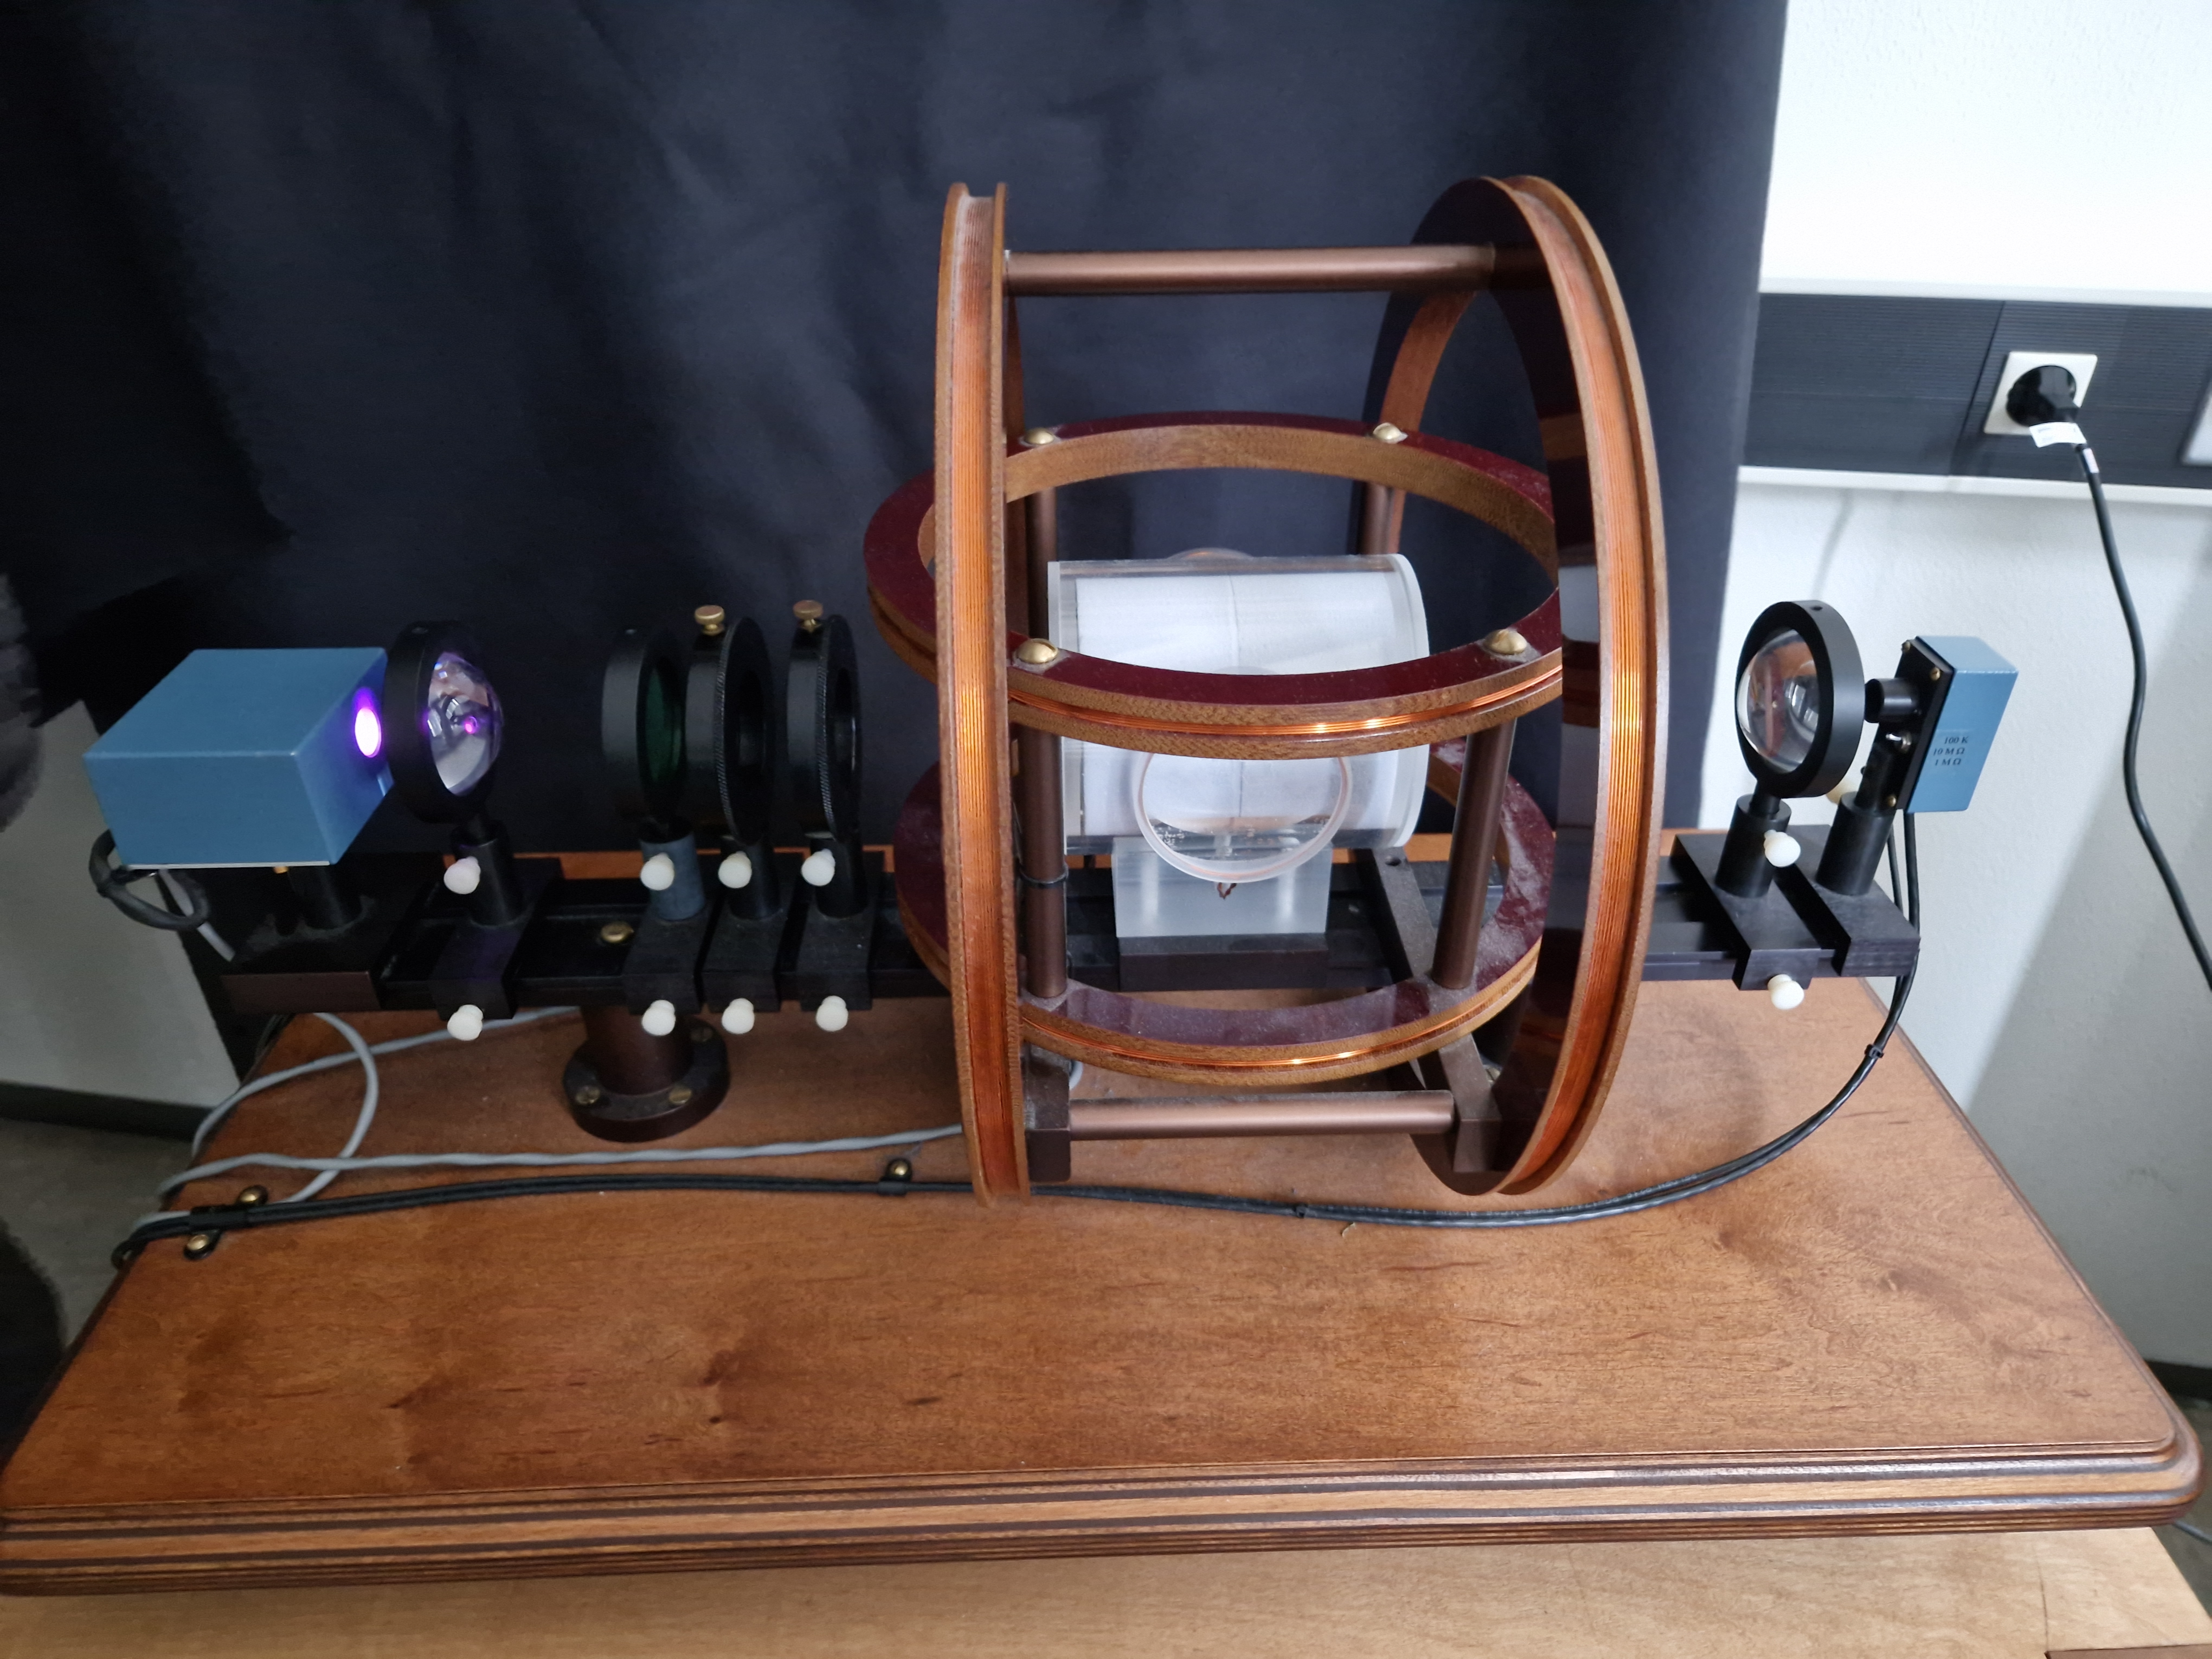
\includegraphics[width=6cm]{figures/aufbau.jpg}}}%
    \qquad
    \subfloat[\centering]{{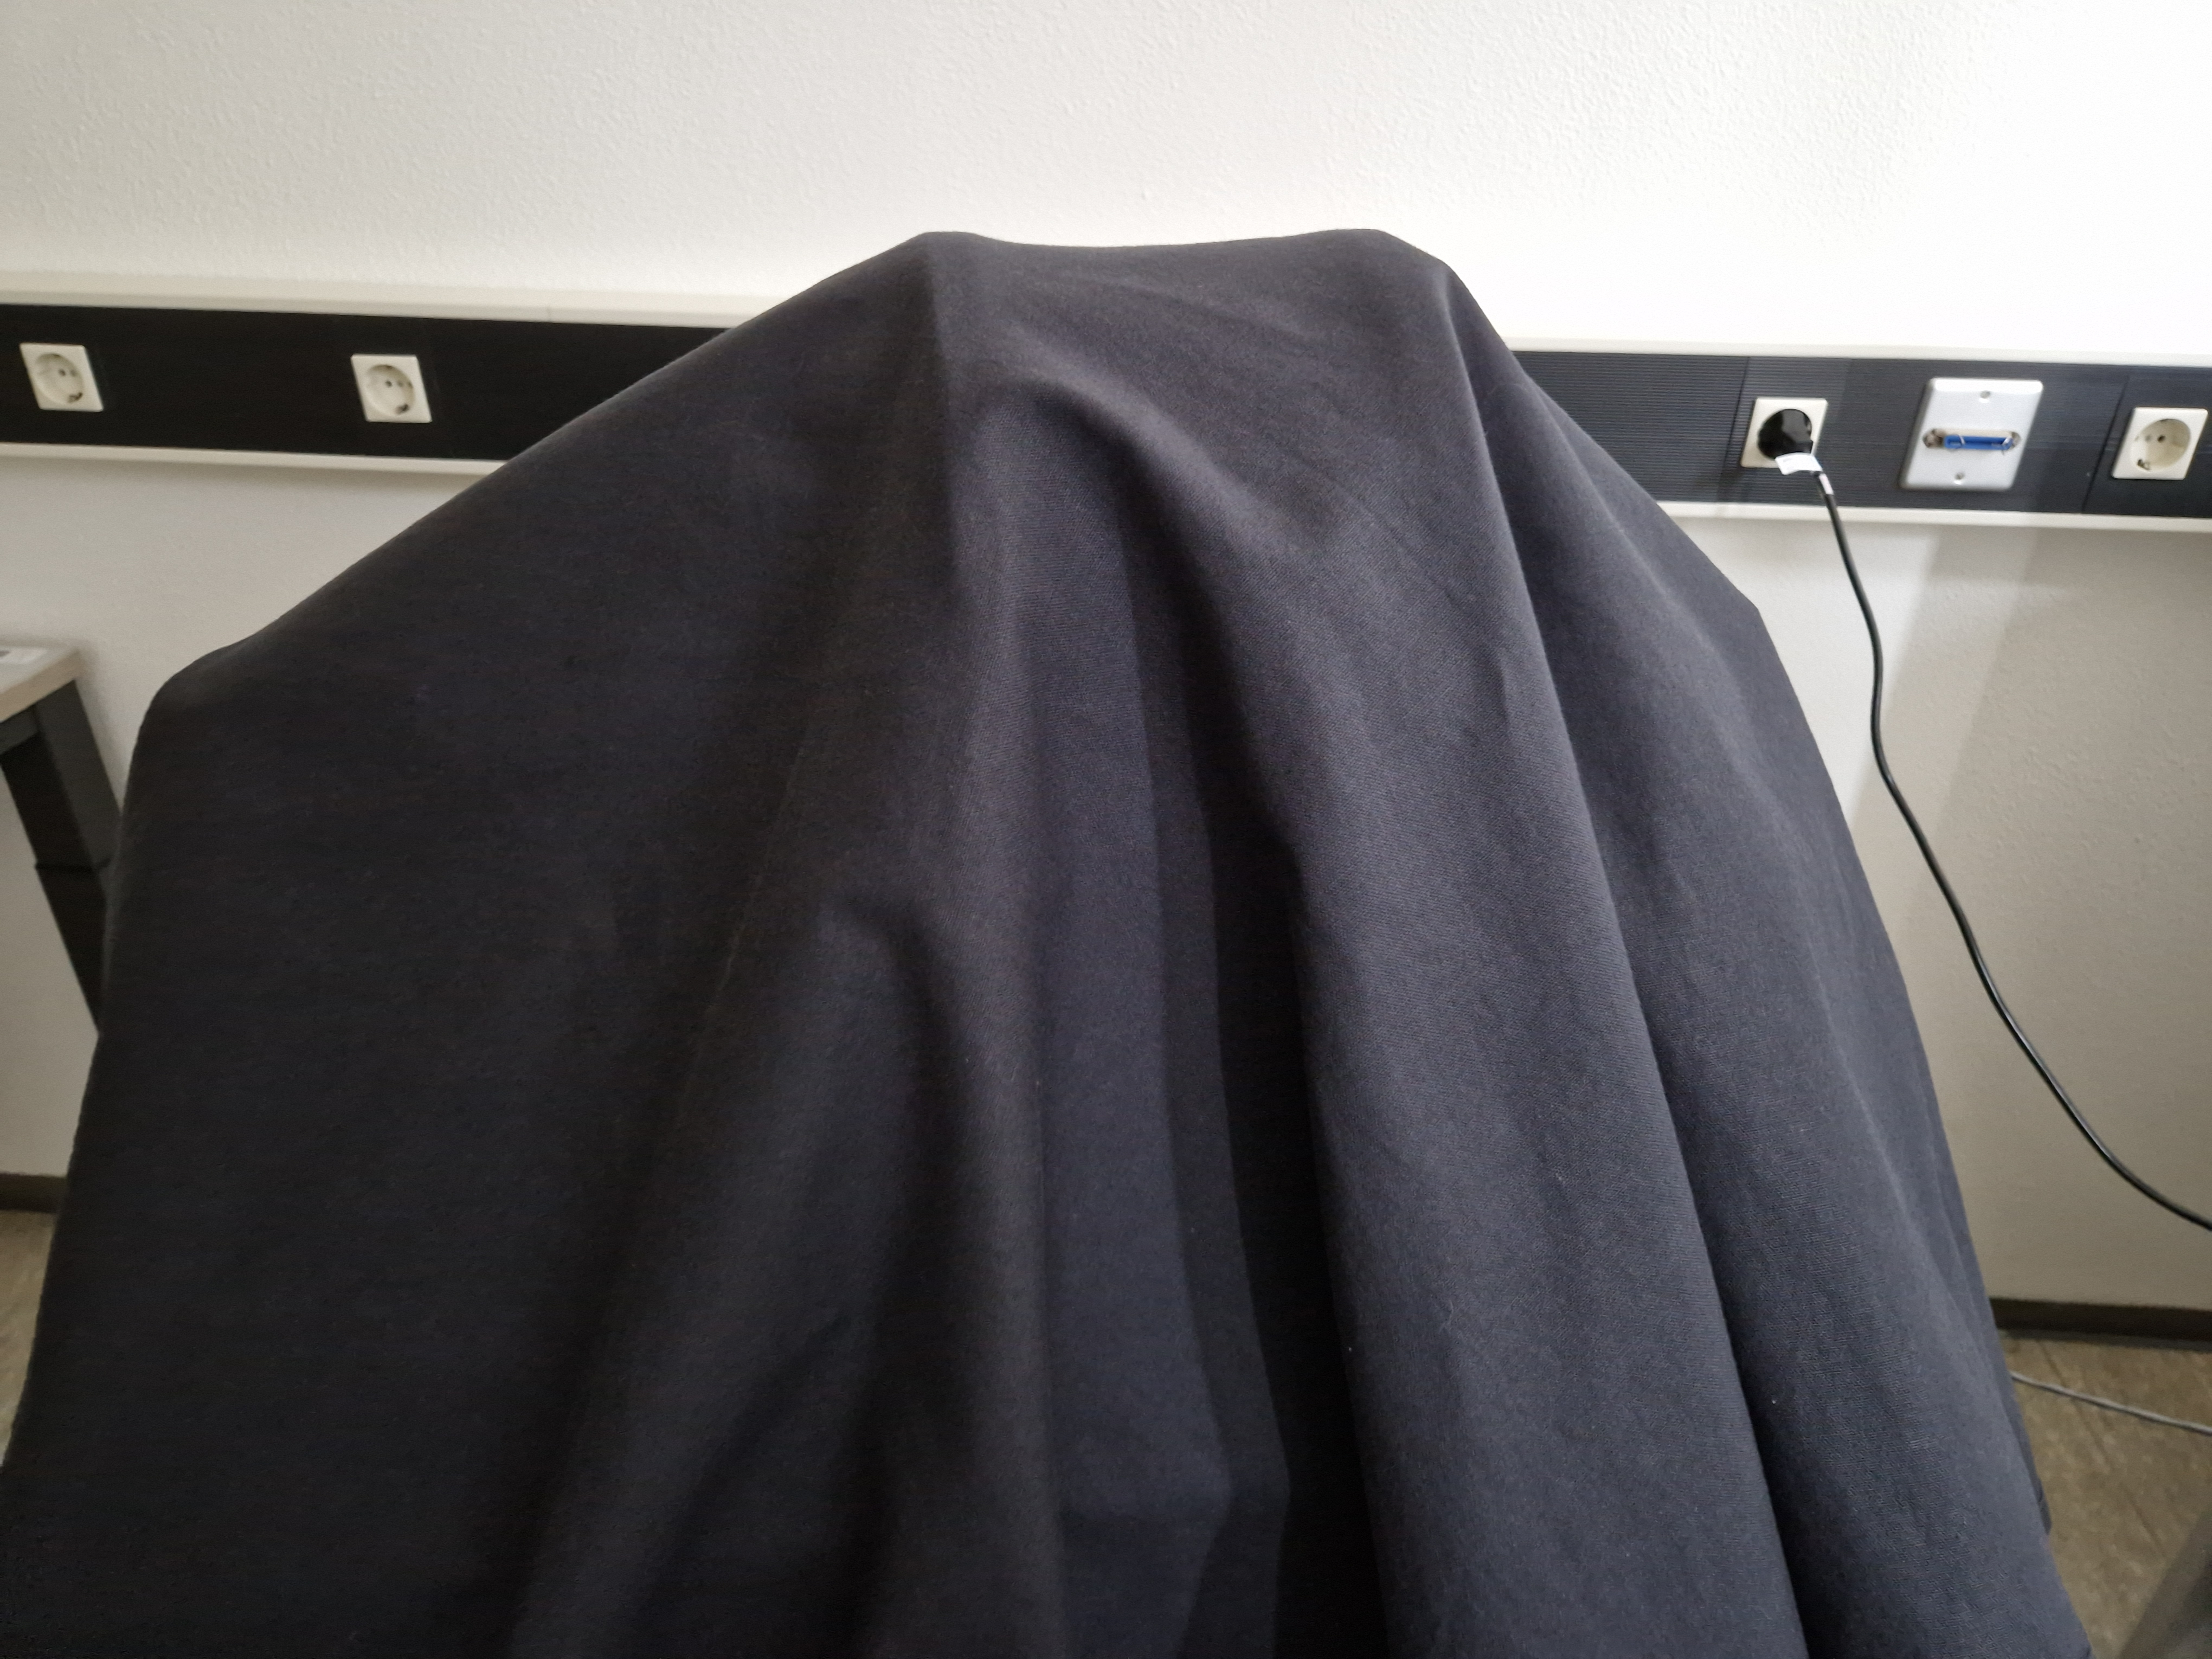
\includegraphics[width=6cm]{figures/aufbau_verdeckt.jpg}}}%
    \caption{Es ist der Aufbau des Versuches dargestellt, links ohne den Lichtschutz, rechts mit Lichtschutz.}
    \label{fig:aufbau}
\end{figure}

Zu Beginn muss das existierende Erdmagnetfeld kompensiert werden.
Dazu wird die vertikal wirkende Helmholtz-Spule angeschaltet und die Stromzufuhr manuell so geregelt, dass der Detektor ein minimales Signal bei ausgeschaltetem RF-Feld ausgibt.
Das ist der Fall, wenn die Vertikalkomponente des Magnetfeldes kompensiert wurde.\\
Damit der Detektor-output ein weiteres Minimum erreichen kann, soll die Apparatur gedreht werden, bis auch die Horizontalkomponenten des Erdmagnetfelds verschwinden.

\subsection{Landefaktoren und horizontales Erdmagnetfeld}
Zur Bestimmung der Horizontalkomponente des Erdmagnetfelds wird der RF-Generator angeschaltet und eine Frequenz von \SI{100}{\kilo\hertz} bis \SI{1}{\mega\hertz} in \SI{100}{\kilo\hertz}-Schritten angelegt.
Zusätzlich wird mit einem Frequenzgenerator eine \SI{100}{\kilo\hertz}-Sinusspannung an die Steuerapparatur angeschlossen, damit die RF stimulierten Resonanzen auf dem Oszilloskop sichtbar werden.
Da das geheizte Rubidium-Gas aus zwei Isotopen besteht, sind auf dem Bildschirm des Oszilloskops auch zwei korrespondierte Peaks zu sehen.
Dies sind die Resonanzpositionen, an denen das kombinierte Magnetfeld der Sweep-Spule und der horizontalen Helmholtz-Spule ausgelesen wird.
Aus der Steigung der sich so ergebenden Geraden für den gegebenen Frequenzbereich, lassen sich gemäß \autoref{eq:zeeman_frequenz} die Landé-Faktoren berechnen.
\subsection{Kernspin, Isotopenverhältnis und quadratischer Zeeman-Effekt}
Aus den Landé-Faktoren wird der Kernspin der jeweiligen Isotope bestimmt und aus der Höhe der Peaks auf dem Oszilloskop wird das Isotopenverhältnis abgelesen.
Zudem soll der quadratische Zeeman-Effekt für die verwendeten Magnetfelder abgeschätzt werden.
\subsection{Rabi-Oszillationen}
\label{sec:rabi}
Um die Rabi-Oszillationen sichtbar zu machen, wird eine Rechteckspannung mit \SI{5}{\hertz} an die Steuerapparatur angeschlossen.
Nach Justierung des Oszilloskops ist eine exponentiell ansteigende Kurve, gefolgt von gedämpften Oszillationen zu sehen.
Die Amplitude des RF-Generators wird nun in kontinuierlichen Schritten bis \SI{10}{\volt} erhöht und für jede Amplitude die Periode der Rabi-Oszillationen am Oszilloskop abgelesen.
Abschließend wird die Periode gegen die RF-Amplitude graphisch dargestellt und durch eine Hyperbel gefittet.
Das Verhältnis aus den Faktoren des Fits gibt an, wie viel die Messung vom theoretischen Wert abweicht.
\newpage
\section{Auswertung}
\label{sec:auswertung}
\subsection{Landefaktoren}
Um optimale Ergebnisse zu erzielen muss zunächst die vertikale Komponente des Erdmagnetfeldes komepensiert werden da diese einen störenden Offset in den Daten verursacht.
Dafür wird, wie in Abschnitt \ref{sec:durchfuerung} beschrieben, das Magnetfeld der vertikale Spule solange varriert bis sich drei schmaller Peaks zeigen.
Der Größte davon korrespondiert zu der vollen Komepensation des Magnetfelds in eine Richtung.
Die anderen Peaks treten dann auf wenn die Zeeman-Aufspaltung gleich der RF-Spulen Energie ist.
Es wird die B-Feld Stärke verwendet bei der die Peaks am schmallsten sind.
Dies wird bei einem Wert von $B_\text{v} = \SI{3.45e-5}{\tesla}$ erreicht.
Danach wird mit Hilfe einer horizontalen Sweep Spule die Magnetfeld Stärke in dieser Raumrichtung geändert.
Die horizontale B-Feldstärke in den Peaks wird dann gegen die angelegte RF-Spulelenfrequenz geplottet.
Der resultierende Plot ist in Abbildung \ref{fig:lande} zu sehen.
Da beiden Isotope unterschiedliche Landefaktoren haben unterscheidet sich auch die Steigung der Geraden die durch das Auftragen der $B$ und $f$ Werte entsteht.
Um nun das Erdmagnetfeld in Horizontal Richtung zu bestimmen wird für beide Isotope eine Ausgleichsgerade nach der Gleichung 
\begin{equation}
    B(f) = a\cdot f + b
\end{equation}
angefertigt.
Die berechneten Parameter für das erste Isotop sind dabei 
\begin{align*}
    a_\text{Iso1} & = \SI{0.495(7)}{\tesla\Hz} \\
    b_\text{Iso1} & = \SI{2.23(13)e-05}{\tesla}
\end{align*}
und die für das zweite Isotop sind
\begin{align*}
    a_\text{Iso2} &= \SI{0.3317(17)}{\tesla\Hz}\\ 
    b_\text{Iso2} &= \SI{2.34(7)e-05}{\tesla} \, .
\end{align*}
Der Wert $b$ gibt nun die jeweilige horizontale Erdmagnetfeldstärke an.
\begin{figure}
    \centering
    \includegraphics[width=\textwidth]{content/plots/landefaktor.pdf}
    \caption{Die Abbildung zeigt die B-Felder der negativen Peaks beider Isotope die gegen die RF-Spulelenfrequenz aufgetragen wird.
    Es ist zu erkennen das die resultierenden Geraden unterschiedliche Steigungen haben.
    In der Abbildung sind zudem zwei Ausgleichsgerade zu sehen die in die Messwerte beider Isotope hineingesetzt werden.}
    \label{fig:lande}
\end{figure}
Aus den Steigungen $a_\text{Iso1}$ und $a_\text{Iso2}$ können nun die beiden Landefaktoren der Isotope berechnet werden.
Dafür wird Gleichung \eqref{eq:zeeman_frequenz} genutzt wodurch sich die Landefaktoren
\begin{align*}
    g_\text{Iso1} &= \SI{0.4950(70)}{}\\
    g_\text{Iso2} &= \SI{ 0.3317(17)}{}
\end{align*}
ergeben.
\subsection{Kernspin}
Aus den zuvor berechneten Landefaktoren kann nun der Kernspin beider Isotope bestimmt werden.
Da bei den genutzt Isotopen gilt, dass 
\begin{align*}
    J, S &= \frac{1}{2}\\
    L &= 0
\end{align*}
kann mithilfe der Gleichung \eqref{eq:landefaktor} der Kernspin werden, da dies die letzte unbekannte Größe ist.

So ergeben sich für die oben genannten Werte des Landefaktors die Kernspins 
\begin{align*}
    I_\text{Iso1} &= \SI{1.522(30)}{}\\
    I_\text{Iso2} &= \SI{2.515(15)}{} \, .
\end{align*}

In Quelle \cite{pdf_anleitung} ist angeben, dass das Isotop {$^{85}\text{Rb}$ einen Kernspin von $\frac{5}{2}$} und das Isotop $^{87}\text{Rb}$ einen Kernspin von $\frac{3}{2}$ hat.
Damit erschließt sich, dass Isotop 1  $^{87}\text{Rb}$ ist und Isotop 2 $^{85}\text{Rb}$ entspricht.

\subsection{Isotopenverhältnis}
Für die Bestimmung des Isotopenverhältnis wird die Abbildung \ref{fig:isotop} in 'inkscape' \cite{Inkscape} eingefügt um die Breite der Peaks in Anzahl von Pixeln zu zählen.

\begin{figure}
    \centering
    \includegraphics[width=0.5\textwidth]{Data/isotope.jpeg}
    \caption{Ein Foto der Messung die mit einem Oszilloskop aufgenommen wird.
    Diese trägt das angelegte Magnetfeld gegen den Strom der Photodiode auf.
    Es sind drei negative Peaks zu sehen.
    Von links nach rechts korrespondieren diese zu dem Nulldurchgang des angelegte Magnetfeldes, dem 1. Isotop und dem zweiten Isotop.}
    \label{fig:isotop}
\end{figure}
Für den linken negativen Peak wird eine Anzahl von $10.93$ Pixeln und für den Rechten $21.971$ Pixel gezählt.
Damit stellt sich ein Isotopenverhältnis von 
\begin{align*}
    ^{87}\text{Rb} \, &\widehat{=}\, 33.22\% \\
    ^{85}\text{Rb} \, &\widehat{=}\, 66.77\%
\end{align*}
ein.

\subsection{Quadraitsche Zeemanaufspaltung}
Um die Stärke der maximalen quadratischen Zeemanaufspaltung bei gegebenen Versuchsaufbau abzuschätzen wird bei der Resonanzfrequenz von $\SI{100}{\k\Hz}$ das größt mögliche Magnetfeld genutzt.
Aus Quelle \cite{pdf_anleitung} ist zu entnehmen, dass für $^{85}\text{Rb}$ $m_\text{F} = 3$ ist und für $^{87}\text{Rb}$ $m_\text{F} = 2$ ist.
Daraus kann nun mit Gleichung \eqref{eq:zeemanaufspaltung} die maximale Zeemanaufspaltung berechnet werden.
Die Aufspaltungen zu den jeweiligen Magnetfeldstärken sind
\begin{align*}
    \Delta E_\text{Iso1} = \SI{4.77(7)}{\eV} & B=\SI{0.1665}{\m\tesla} \\
    \Delta E_\text{Iso2} = \SI{4.557(23)}{\eV} & B=\SI{0.2377}{\m\tesla}  \, .
\end{align*}

\subsection{Rabioszillation}
Die Messwerte für diesen Abschnitt werden gemäß das Ablaufs der in Abschnitt \ref{sec:rabi} beschrieben wird, aufgenommen.
Danach wird die Periodendauer $T$ gegen die RF-Amplitude $A_0$ aufgetragen.
Der resultierende Plot ist in Abbildung \ref{fig:rabi} zu sehen.
\begin{figure}
    \centering
    \includegraphics[width=\textwidth]{content/plots/periodendauer.pdf}
    \caption{Die Periodendauer der Rabioszillation wird gegen die angelegte RF-Amplitude aufgetragen.
    Zudem wird eine Ausgleichsrechung durchgeführt dessen Fit ebenfalls in der Grafik zu sehen ist.}
    \label{fig:rabi}
\end{figure}
An die Messwerte beider Isotope wird ein Fit gemäß der Gleichung 
\begin{equation*}
    T(A_0) = a + \frac{b}{A_0}
\end{equation*}
angepasst.
Die berechneten Parameter für Isotop 1 sind 
\begin{align*}
    a_\text{Iso1} &= \SI{0.132(23)e-3}{\ms}\\
    b_\text{Iso1} &= \SI{3.94(5)e-3}{\V\ms} \, .
\end{align*}
Für Isotop 2 ergeben sich die Parameter 
\begin{align*}
    a_\text{Iso2} &= \SI{0.145(26)}{\ms}\\
    b_\text{Iso2} &= \SI{6.01(6)}{\V\ms} \, .
\end{align*}
Der gefragt Quotient aus $\frac{b_\text{Iso2}}{b_\text{Iso1}}$ kann nun berechnet werden.
Dieser beträgt 
\begin{align*}
    \frac{b_\text{Iso2}}{b_\text{Iso1}} &= \SI{1.525(26)}{} \, .
\end{align*}

\section{Diskussion}
\label{sec:diskussion}
In diesem Teil des Protokolls werden die Ergebnisse mit den theoretischen Werten verglichen um mögliche Fehlerquellen erläutert, die zu Abweichungen zwischen Theorie und Experiment führen.
\subscetion{invertierter Linearverstärker}
Zunächst wird für den Linearverstärker die Abweichung der Verstärkung berechnet, diese ist in Tabelle \ref{tab:lin_disk} zu sehen.
Die Abweichung liegen alle unter $2\,\%$ und sind damit im experimentellen Rahmen.
\begin{table}
    \centering
    \begin{tabular}{cccc}
        \toprule
        &Messung 1 & Messung 2 & Messung 3\\
        \midrule
        Mittelwert $\bar{V}'$ & $\SI{93.600(2100)}{}$ &  $\SI{2.080(1)}{} $&  $\SI{4.680(50)}{} $ \\
        theoretische Verstärkung $V_\text{theo}'$ & 100 & 2.126 & 4.680 \\
        Abweichung$\,\%$ & $\SI{6.4(21)}{} $& $\SI{2.2(1)}{}$ & $\SI{0.0(10)}{}$ \\
        \botoomrule
    \end{tabular}
    \caption{Die Abweichung der theoretischen Verstärkung zur experimentellen Verstärkung.}
    \label{tab:lin_disk}
\end{table}
Die Verstärkung der invertierenden Linearverstärkers zeigt das erwartete Plateu für niedrige Frequenz.
Ab einer Grenzfrequenz, die mit der theoretischen Grenzfrequenz übereinstimmt, fällt die Verstärkung exponentiell bis auf 0 ab.
\subsection{Umkehr Integrator und invertierender-Differenzierer}
Der Umkehrintegrator und der invertierender-Differenzierer bilden wie erwartet die Stammfunktion beziehungsweise die Ableitung des Eingangssignal, was in den Abbildung \ref{fig:umkehr_oszi} und \ref{fig:dif_oszi} zu erkennen ist.
Die Ausgangsspannung weist das ewartete Verhalten auf und eine Ausgleichsgerade konnte gut an die Messwerte gelegt werden.
\subsection{Schmitt-Trigger}
Wie erwartet springt die Ausgangsspannung des Schmitt-Triggers ab einer Grenzamplitude auf $\approx \SI{30}{\V}$.
Die Abweichung der experimentellen Grenzamplitude $U_\text{Schmitt} &= \SI{3.26}{\V}$ zu der theoretischen $U_\text{Schmitt,theo} &= \SI{2.91(5)}{\V}$ beträgt $Abw = \SI{12.03(19)}{}\%$.
Der Schmitt-Trigger hat damit wie erwartet funktioniert und weißt nur gewisse Abweichung zwischen Experiment und Theorie auf.
Diese kann mit den schlechten Kontakten der Steckplatine begründert werden, die zu einem höheren Widerstand geführt haben können.
\subsection{Signalgenerator}
Der Generator hat das erwartet Dreiecksspannungs Signal ausgegeben, allerdings hatte dieses mit $U_\text{a,2} &= \SI{5.20(5)}{\V}$ eine höhere Spannung als erwatet $U_\text{a,2,theo} &= \SI{2.77(5)}{\V}$.
Die Abweichung des experimentellen Wertes zum theoretischen beträgt $Abw = \SI{87.73(34)}{}\%$.
Es ist wahrscheinlich, dass auch hier die Steckplatine für einen höheren Widerstand gesorgt hat, weswegen das Ausgangssignal verfälscht wurde.
\\\\
Die Schaltungen könnten durch gelötete Kontakt verbessert werden, da diese weniger Fehleranfällig sind und nur einen sehr kleinen Widerstand haben.
Dies würde natürlich zu einem größeren Aufwand führen.
Zudem schienen die Operationsverstärker teilweise kaputt zu sein, was ebenfalls zu Fehlern geführt haben könnte.


\appendix

\begin{table}[H]
  \centering
  \caption{Measured data}
  \resizebox{!}{10cm}{%
  \csvreader[tabular=c|c|c|c|c,
  head=false, 
  table head= $\Delta t$ in s & shield resistance in $\Omega$ & probe resistance in $\Omega$ & voltage in \si{\volt} & current in \si{\ampere} \\\midrule,
  late after line= \\]
  {Data/data.csv}{1=\eins, 2=\zwei, 3=\drei, 4=\vier, 5=\five}{$\num{\eins}$ & $\num{\zwei}$ & $\num{\drei}$ & $\num{\vier}$ & $\num{\five}$}}
  \label{tab:data}
\end{table}

\newpage
\printbibliography{}

\end{document}
